\section{Внешние форматы хранения данных}
%\addcontentsline{toc}{section}{Внешние форматы хранения данных}

Файлы для баз данных хранятся в формате CSV (Comma Separated Values) \cite{csv}. В каждом файле присутствует заголовочная строка, показывающая какие данные хранятся в каждом столбце. Данные в столбцах разделяются запятыми.

CSV формат так же применяется для запросов.

Для грузовиков определены следующие столбцы:
\begin{itemize}
	\item id -- идентификационный номер грузовика (int);
	\item brand -- код марки грузовика (int);
	\item capacity -- грузоподъёмность грузовика в тоннах (float);
	\item transportation\_distance -- максимальная дальность перевозки (int).
\end{itemize}

Пример таблицы грузовиков указан на рис. \ref{truck_table}.

\begin{figure}[hpt!]
	\centering
	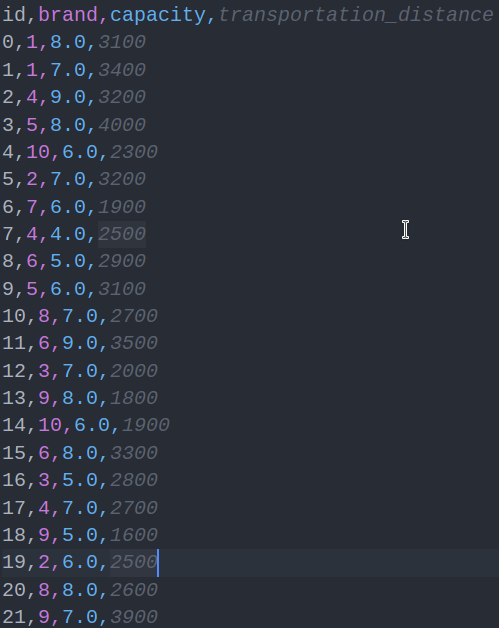
\includegraphics[width=0.5\linewidth]{photo/truck_table}
	\caption{Пример таблицы грузовиков}
	\label{truck_table}
\end{figure}

\newpage
Для водителей определены следующие столбцы:
\begin{itemize}
	\item id -- идентификационный номер водителя (int);
	\item name -- имя водятеля (string);
	\item name -- фамилия водятеля (string);
	\item name -- отчество водятеля (string);
	\item brand\_code -- код разрешённой марки грузовика (int).
\end{itemize}

Пример таблицы водителей указан на рис. \ref{driver_table}.

\begin{figure}[hpt!]
	\centering
	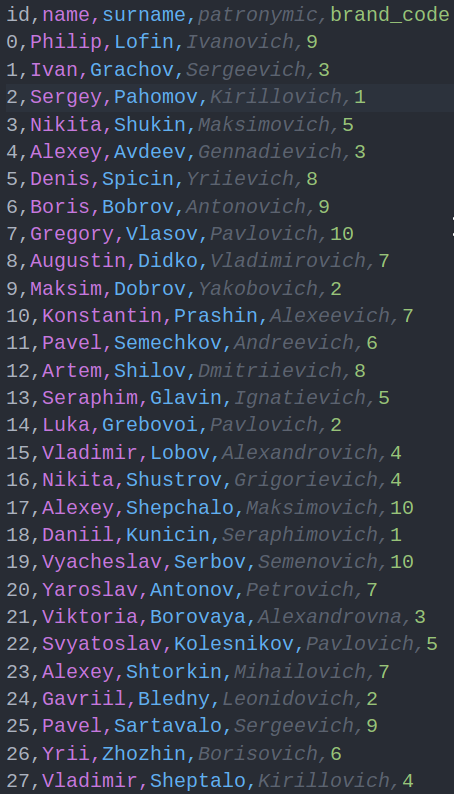
\includegraphics[width=0.5\linewidth]{photo/driver_table}
	\caption{Пример таблицы водителей}
	\label{driver_table}
\end{figure}

\newpage

Для маршрутов определены следующие столбцы:
\begin{itemize}
	\item id -- идентификационный номер маршрута (int);
	\item destination\_code -- код конечного пункта (int);
	\item distance -- длина маршрута в км (int);
	\item loading\_time -- время погрузки/разгрузки в конечных пунктах в ч (int);
	\item drivers -- кол-во водителей (int);
	\item time\_in\_transit -- расчётное время поставки в одну сторону (ч) (int).
\end{itemize}

Пример таблицы маршрутов указан на рис. \ref{route_table}.

\begin{figure}[hpt!]
	\centering
	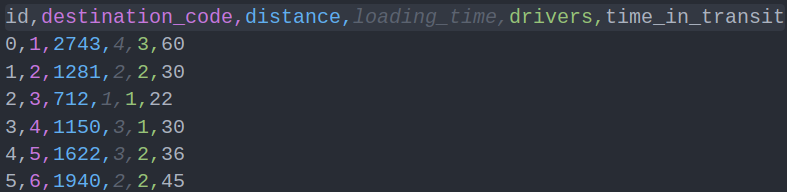
\includegraphics[width=0.8\linewidth]{photo/route_table}
	\caption{Пример таблицы маршрутов}
	\label{route_table}
\end{figure}

Для графика поставок определены следующие столбцы:
\begin{itemize}
	\item start -- время отправки поставки в секундах от 1 янв 1970 00:00 (int);
	\item end -- время возврата грузовика в секундах от 1 янв 1970 00:00 (int);
	\item truck\_id -- идентификационный номер грузовика (int);
	\item drivers\_ids -- идентификационные номера водителей (указываются через пробел)(int).
\end{itemize}

Пример таблицы графика поставок указан на рис. \ref{schedule_table}.

\begin{figure}[hpt!]
	\centering
	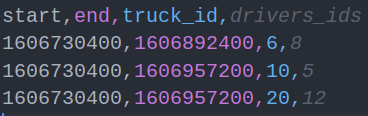
\includegraphics[width=0.8\linewidth]{photo/schedule_table}
	\caption{Пример таблицы графика поставок}
	\label{schedule_table}
\end{figure}

\newpage

Для запросов определены следующие столбцы:
\begin{itemize}
	\item destination -- код конечного пункта (int);
	\item departure\_date -- дата отправки в формате дд.мм.гггг чч:мм (string);
	\item cargo\_weight -- масса груза (float);
	\item truck\_brand -- код предпочитаемой марки грузовика (int).
\end{itemize}

Пример запроса указан на рис. \ref{request_table}.

\begin{figure}[hpt!]
	\centering
	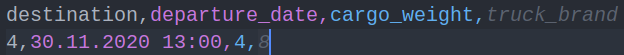
\includegraphics[width=0.8\linewidth]{photo/request_table}
	\caption{Пример запроса}
	\label{request_table}
\end{figure}

Для хранения пароля для доступа к консоли администратора используется обычный текстовый файл, содержащий единственную строку: хэш сумма заданного пароля.

Пример файла с хэшем пароля указан на рис. \ref{hash_example}.

\begin{figure}[hpt!]
	\centering
	
\includegraphics[width=0.8\linewidth]{photo/hash_example}
	\caption{Пример файла с хэшем пароля}
	\label{hash_example}
\end{figure}